\chapter{\textsf{\acronym}}
\section*{Description}
\emph{NUXIS} is a centralized tool that allows the management of available resources on a network. It consists of a Linux distribution pre-installed and configured, which allows you to manage servers' resources.

The \acronym is divided into two functional blocks:

\begin{itemize}
	\item \emph{Central Management} (CM)
    \item \emph{Virtualization Agent} (VA)
\end{itemize}

\begin{figure}[H]
	\begin{center}
	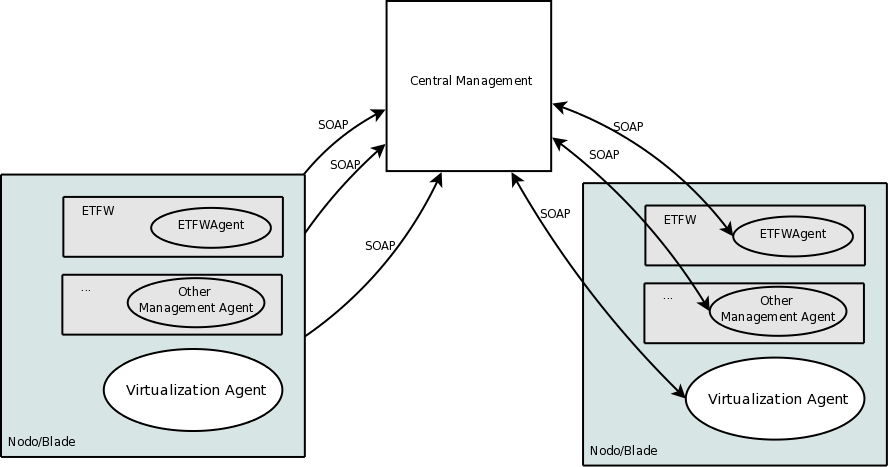
\includegraphics[scale=0.35]{screenshots/etva_blocos.png}
	\caption{\acronym architecture}
	\label{fig:etva_blocos}
	\end{center}
\end{figure}

The CM (Central Management) is the block responsible for managing the entire infrastructure.
The \emph{Virtualization Agents} are responsible for processing the requests between the virtualization server (\emph{node}) and CM.

Within a virtualization server there may be virtual machines with \emph{Management Agents}. These type agent enables the managing of existing services/applications on the virtual machine (see Figure \ref{fig:etva_blocos}).

In the \acronym, there are several virtualization servers (nodes) that communicate with the CM. The initial network configuration is performed, using VLANs through the \emph{One time setup wizard} as shown in Figure \ref{fig:first_time_wizard}.

\begin{figure}[H]
    \begin{center}
	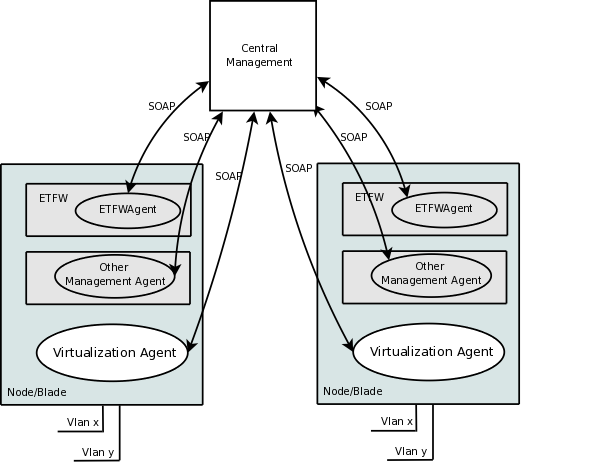
\includegraphics[scale=0.6]{screenshots/etva_enterprise.png}
	\caption{\acronym model}
	\label{fig:etva_enterprise}
	\end{center}
\end{figure}

This user's manual describes the configuration management tool (CM - \emph{Central Management}). 

\pagebreak
\chapter{\textsf{Installation}}
\label{chp:installation}
\section{Enterprise version}

To make installation we need to use CD-ROM with NUXIS ISO installation and boot the server from it.

For enterprise version, we need one server to install manager interface (\emph{Central Management}) and do installation on each virtualization server.

\begin{figure}[H]
	\begin{center}
	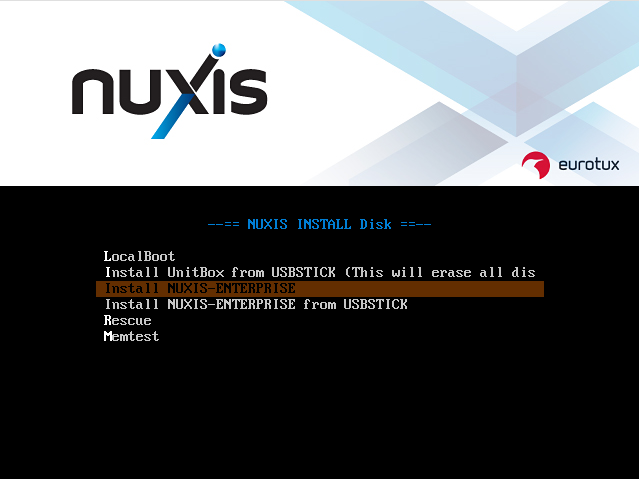
\includegraphics[scale=0.4]{screenshots/install/nuxis/bootmenu.png}
	\caption{Enterprise version menu installation}
	\label{fig:boot_install_screen_enterprise}
	\end{center}
\end{figure}

In both cases, we need boot by CD-ROM and choose \emph{Install NUXIS-ENTERPRISE} option to do the installation step-by-step.

\begin{figure}[H]
	\begin{center}
	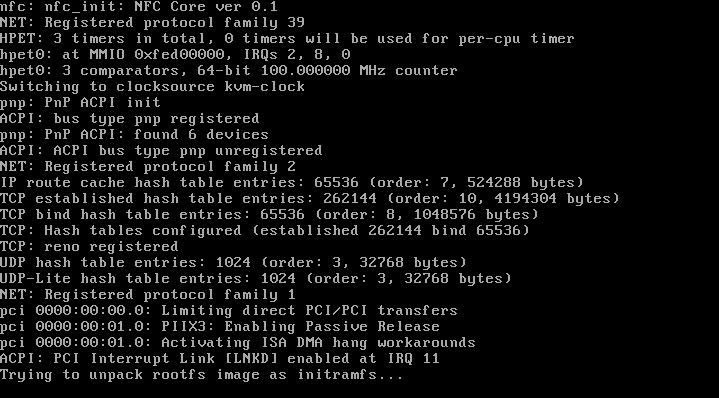
\includegraphics[scale=0.3]{screenshots/install/nuxis/boot_installer.png}
	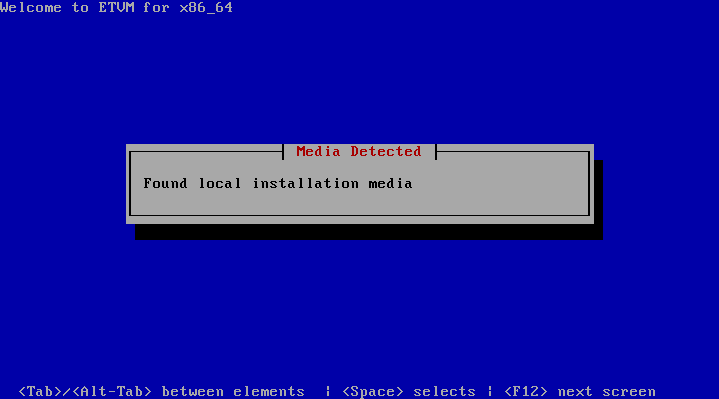
\includegraphics[scale=0.3]{screenshots/install/nuxis/load_installer_01.png}
	%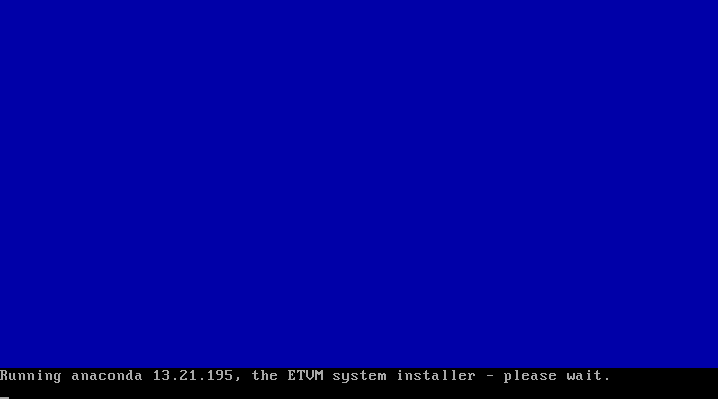
\includegraphics[scale=0.4]{screenshots/install/nuxis/load_installer_02.png}
	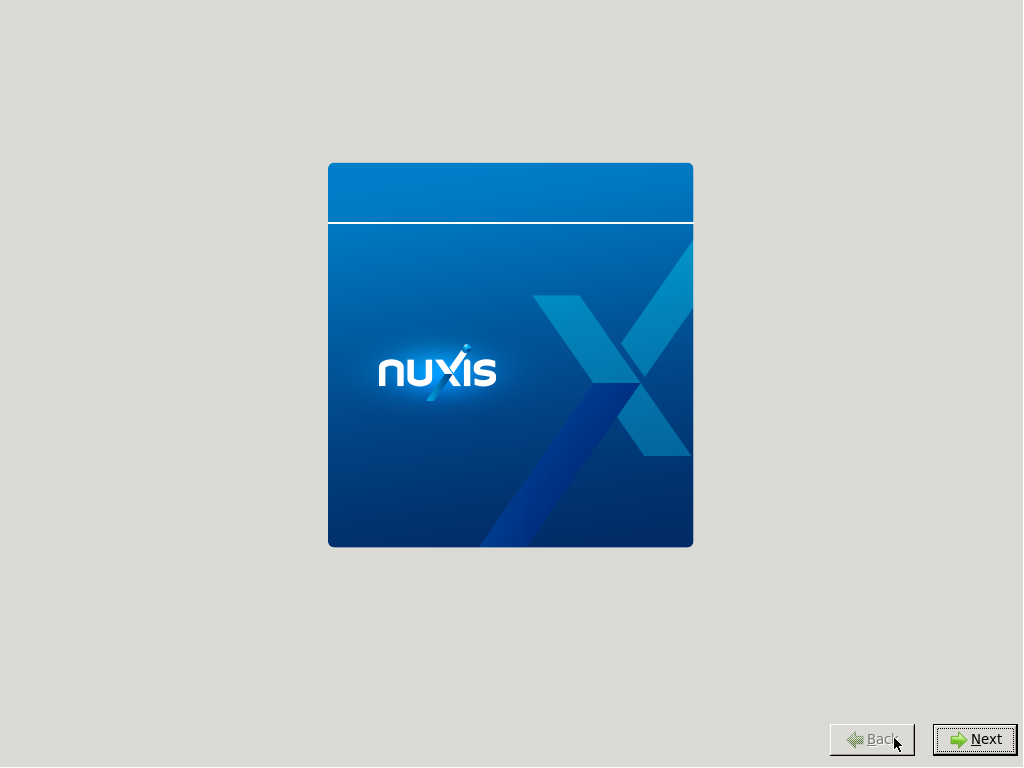
\includegraphics[scale=0.3]{screenshots/install/nuxis/wizard_install_01.png}
    \caption{Enterprise version installation - Startup}
	\label{fig:installation_enterprise_02}
	\end{center}
\end{figure}
\begin{figure}[H]
	\begin{center}
	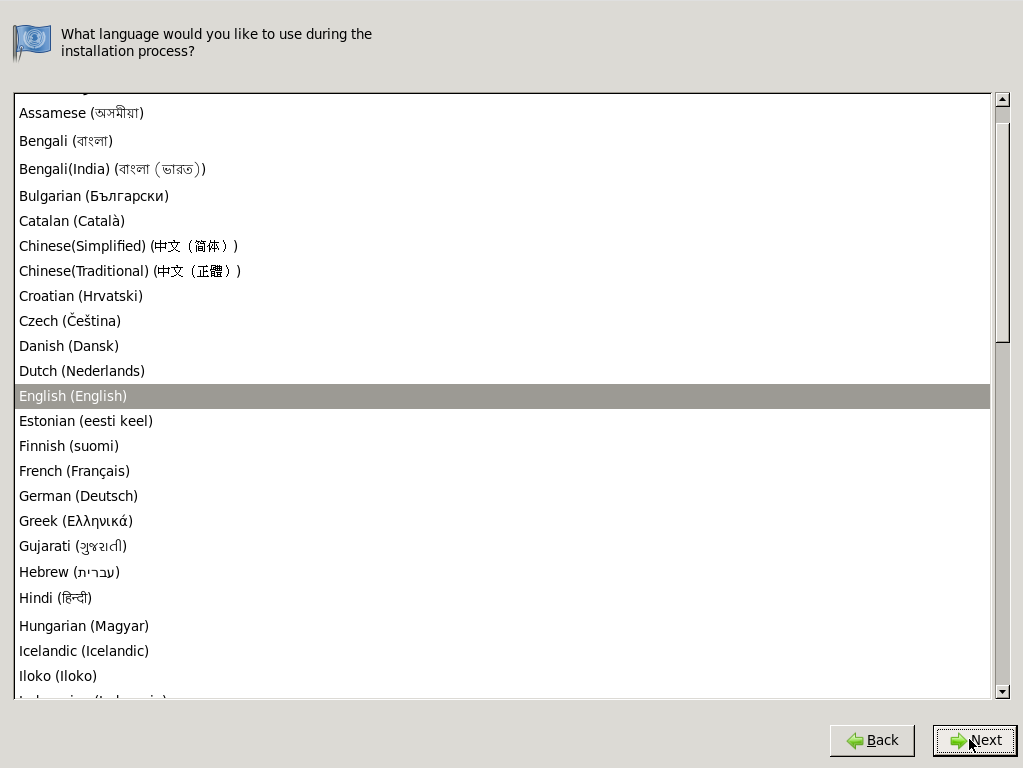
\includegraphics[scale=0.2]{screenshots/install/nuxis/wizard_install_02.png}
	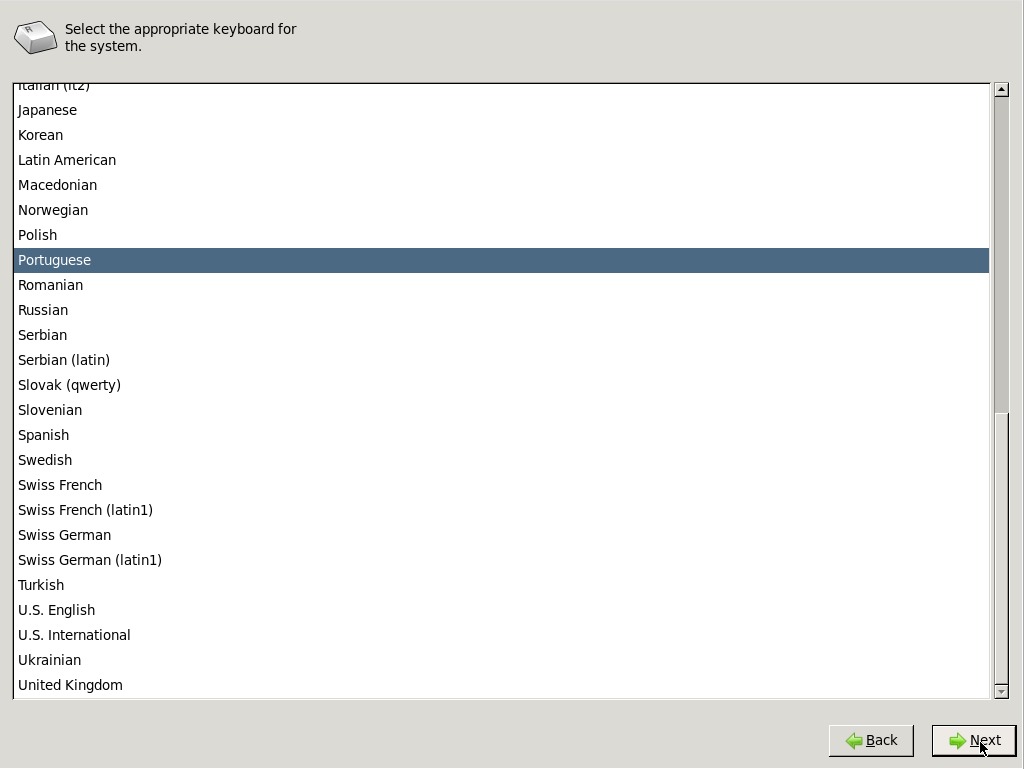
\includegraphics[scale=0.2]{screenshots/install/nuxis/wizard_install_03.png}
	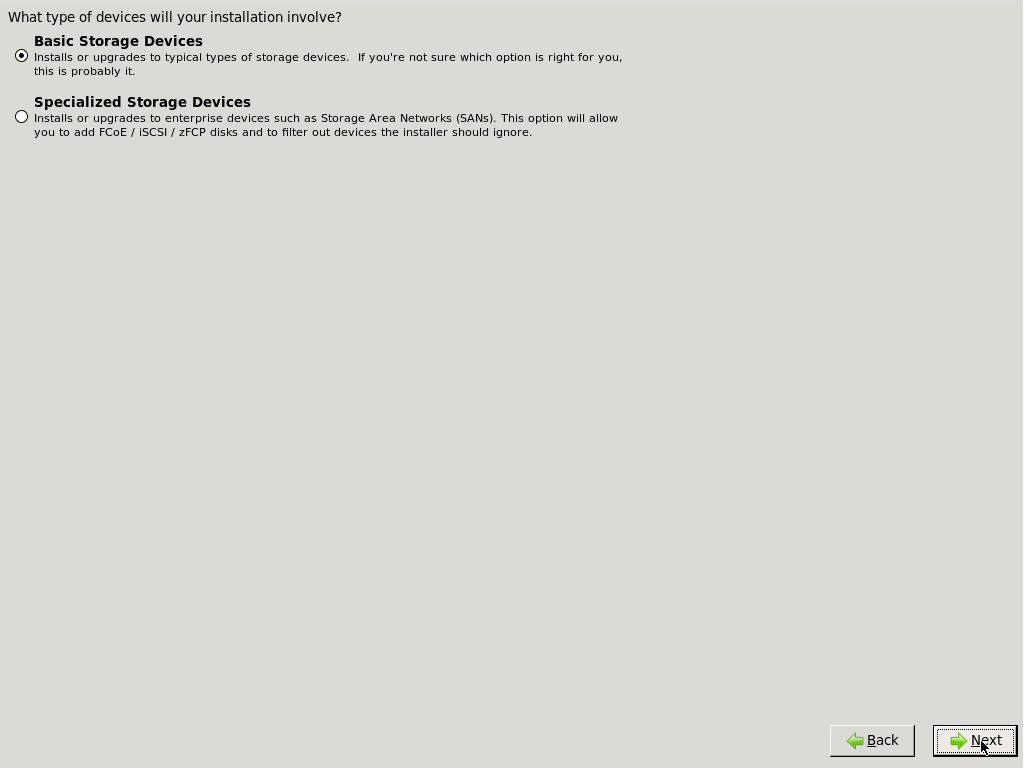
\includegraphics[scale=0.2]{screenshots/install/nuxis/wizard_install_04.png}
	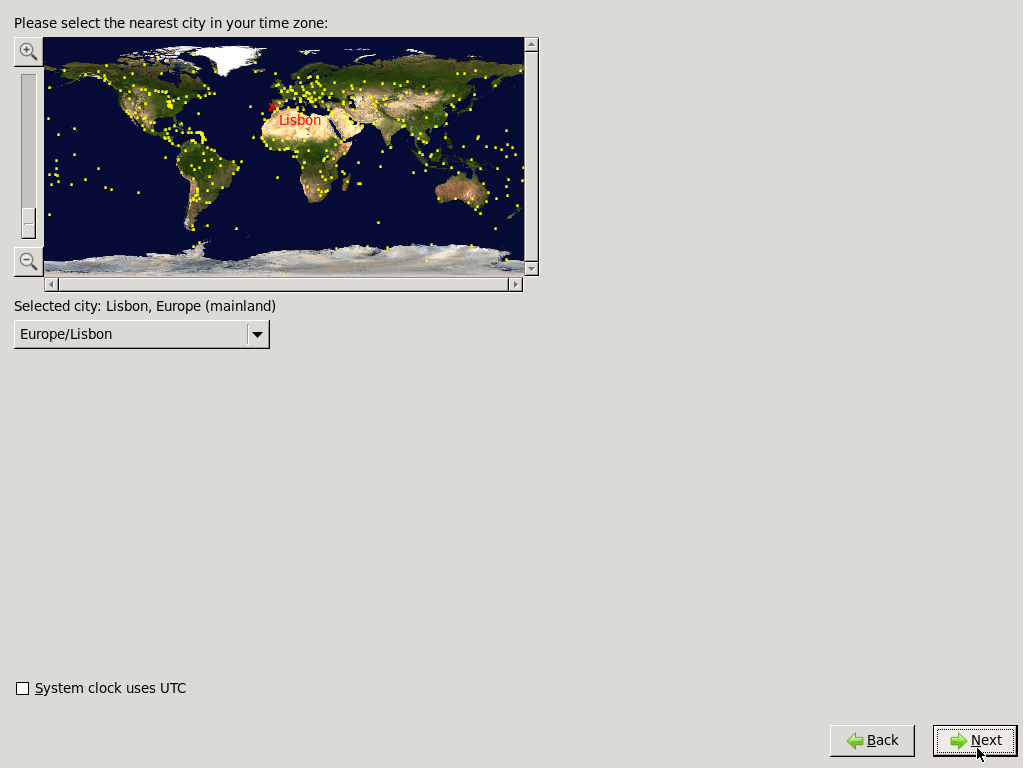
\includegraphics[scale=0.2]{screenshots/install/nuxis/wizard_install_05.png}
	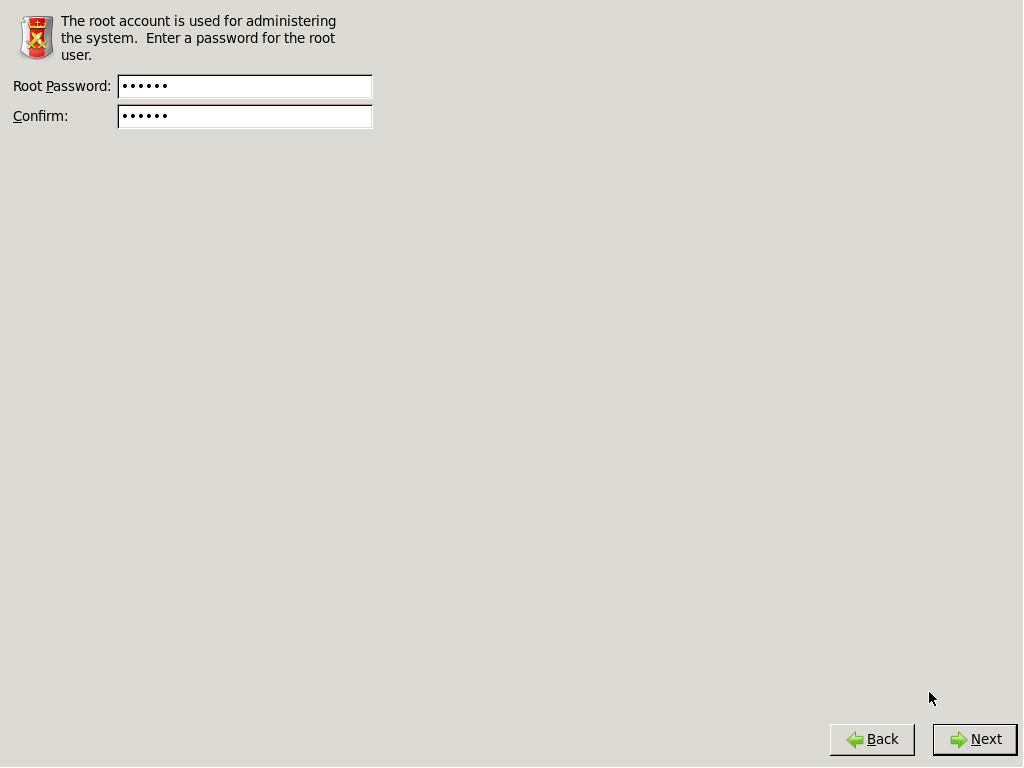
\includegraphics[scale=0.2]{screenshots/install/nuxis/wizard_install_06.png}
	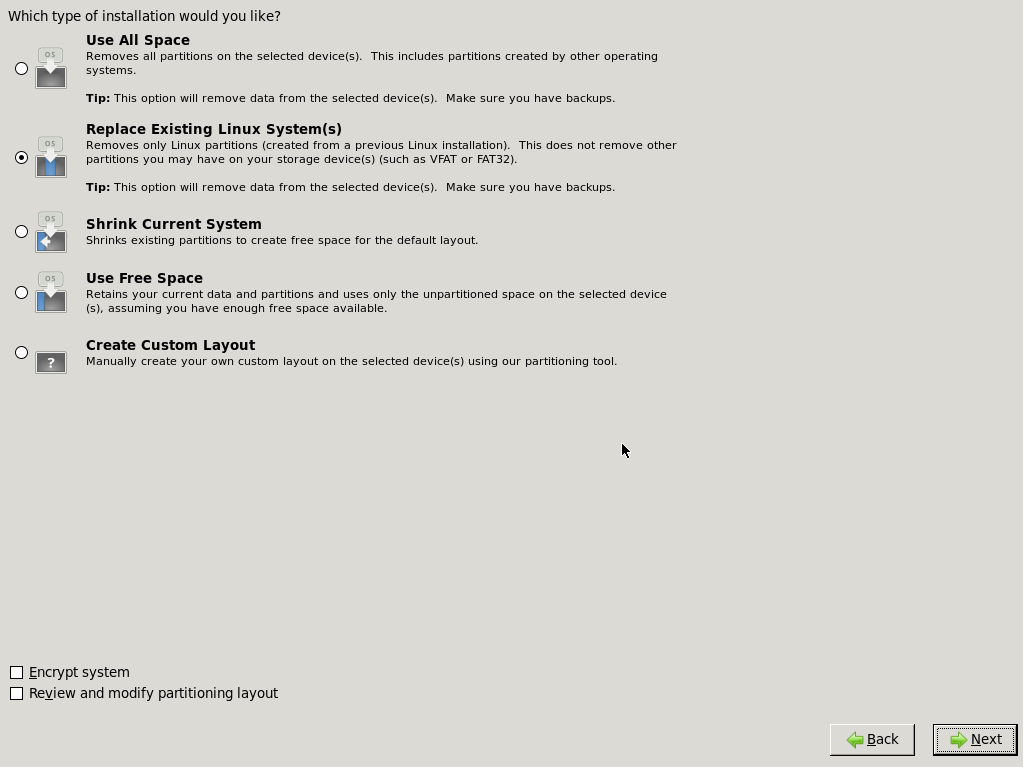
\includegraphics[scale=0.2]{screenshots/install/nuxis/wizard_install_07.png}
    \caption{Enterprise version installation - Configuration}
	\label{fig:installation_enterprise_03}
	\end{center}
\end{figure}
\begin{figure}[H]
	\begin{center}
	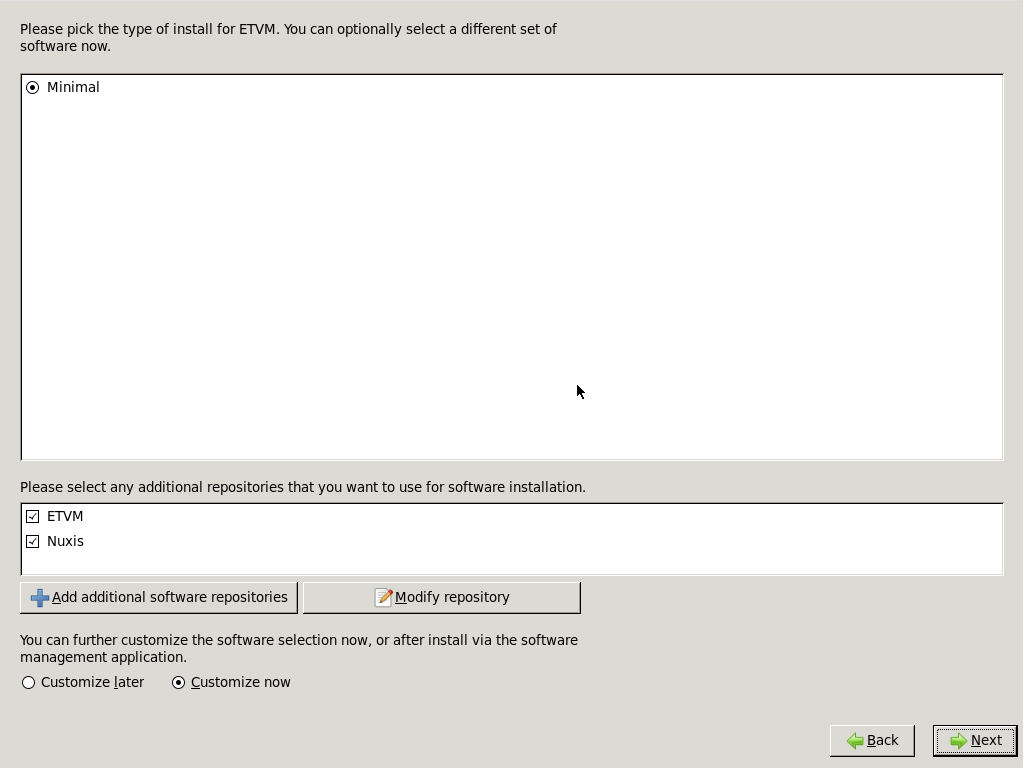
\includegraphics[scale=0.2]{screenshots/install/nuxis/packages_selection_01.png}
	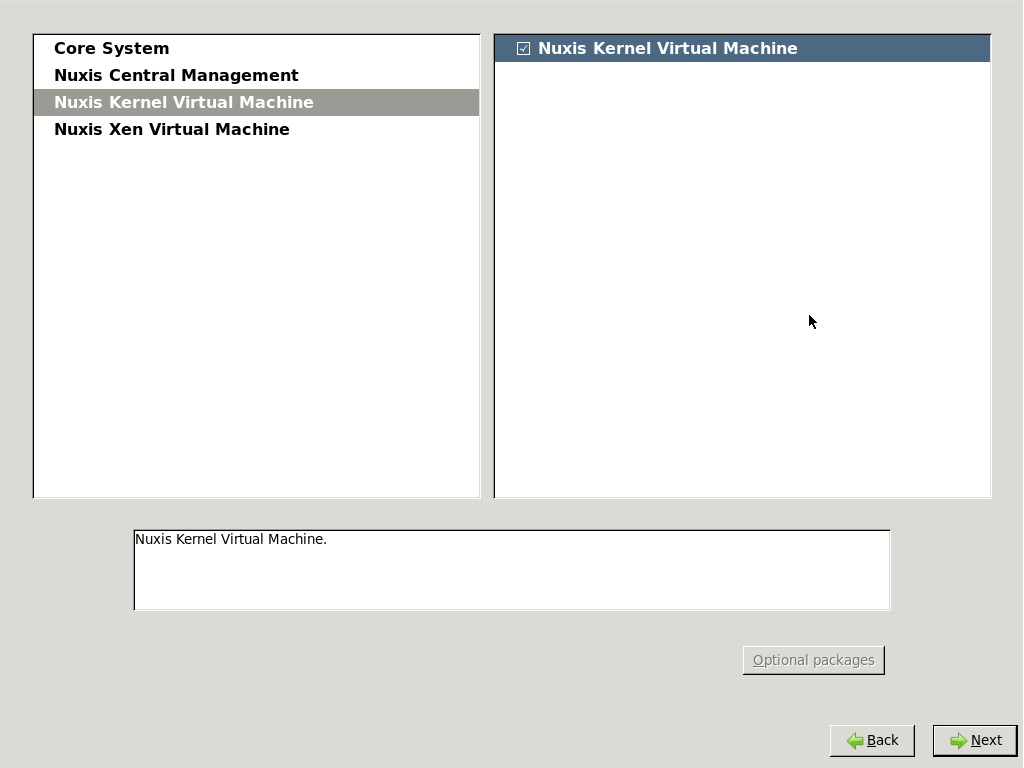
\includegraphics[scale=0.2]{screenshots/install/nuxis/packages_selection_02.png}
    \caption{Enterprise version installation - Packages}
	\label{fig:installation_enterprise_05}
	\end{center}
\end{figure}


On packages interface we should choose \emph{Nuxis Central Management} package for management interface installation, \emph{Nuxis Kernel Virtual Machine} for virtualization server with KVM support and \emph{Nuxis Xen Virtual Machine} for server with XEN support.

\begin{figure}[H]
	\begin{center}
	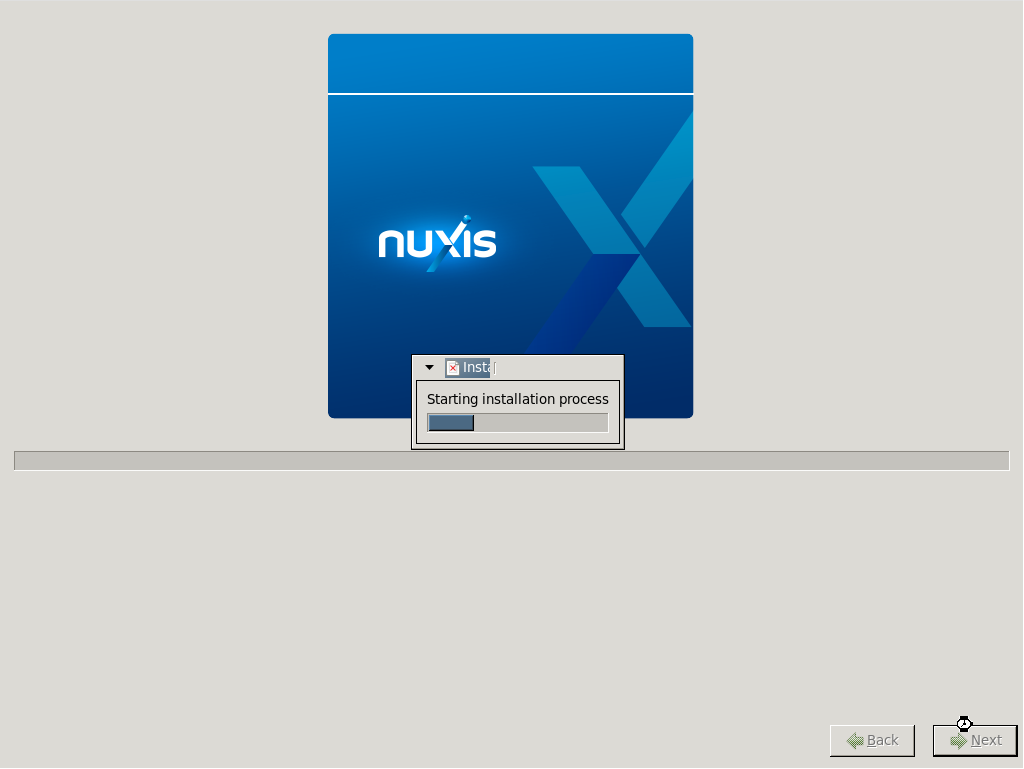
\includegraphics[scale=0.2]{screenshots/install/nuxis/start_install.png}
	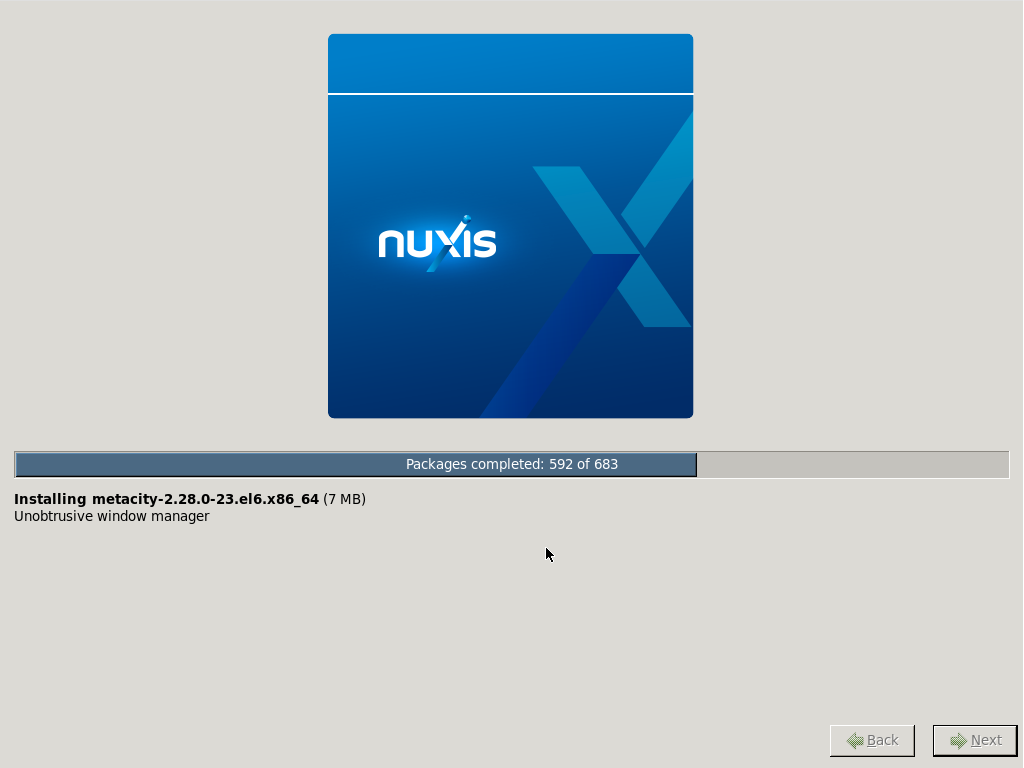
\includegraphics[scale=0.2]{screenshots/install/nuxis/install_progress_02.png}
	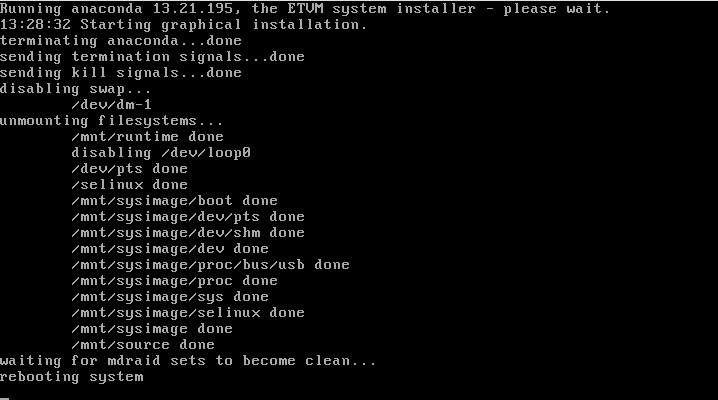
\includegraphics[scale=0.4]{screenshots/install/nuxis/install_reboot.png}
    \caption{Enterprise version installation - complete installation}
	\label{fig:installation_enterprise_06}
	\end{center}
\end{figure}

At the end of installation, we start up the server and proceed to network configuration.

\begin{figure}[H]
	\begin{center}
    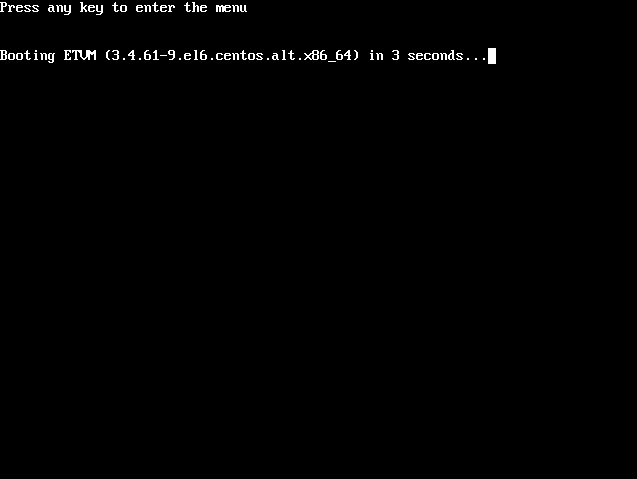
\includegraphics[scale=0.4]{screenshots/install/nuxis/pos_install_bootmenu.png}
    \caption{Configuration after installation - Boot}
	\label{fig:installation_enterprise_pos_01}
	\end{center}
\end{figure}

\begin{figure}[H]
	\begin{center}
    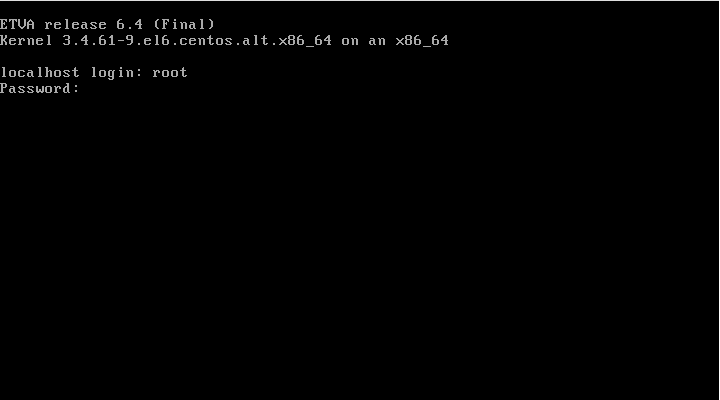
\includegraphics[scale=0.3]{screenshots/install/nuxis/login.png}
    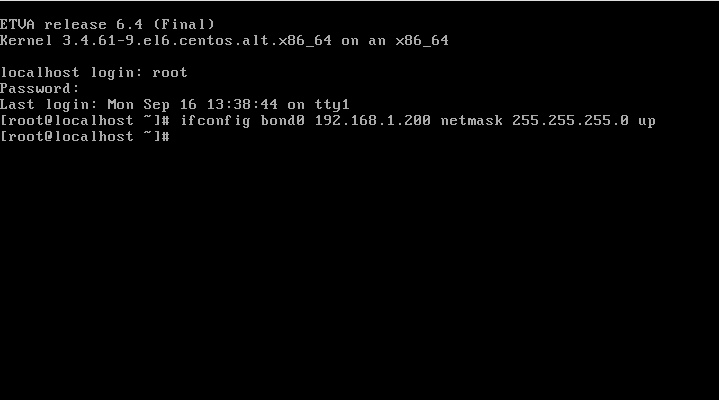
\includegraphics[scale=0.3]{screenshots/install/nuxis/configure_network.png}
    \caption{Configuration after installation - Login and network configuration}
	\label{fig:installation_enterprise_pos_02}
	\end{center}
\end{figure}

For network configuration, we should acess to server console with login \emph{root} and password and set the IP address.

\begin{figure}[H]
	\begin{center}
    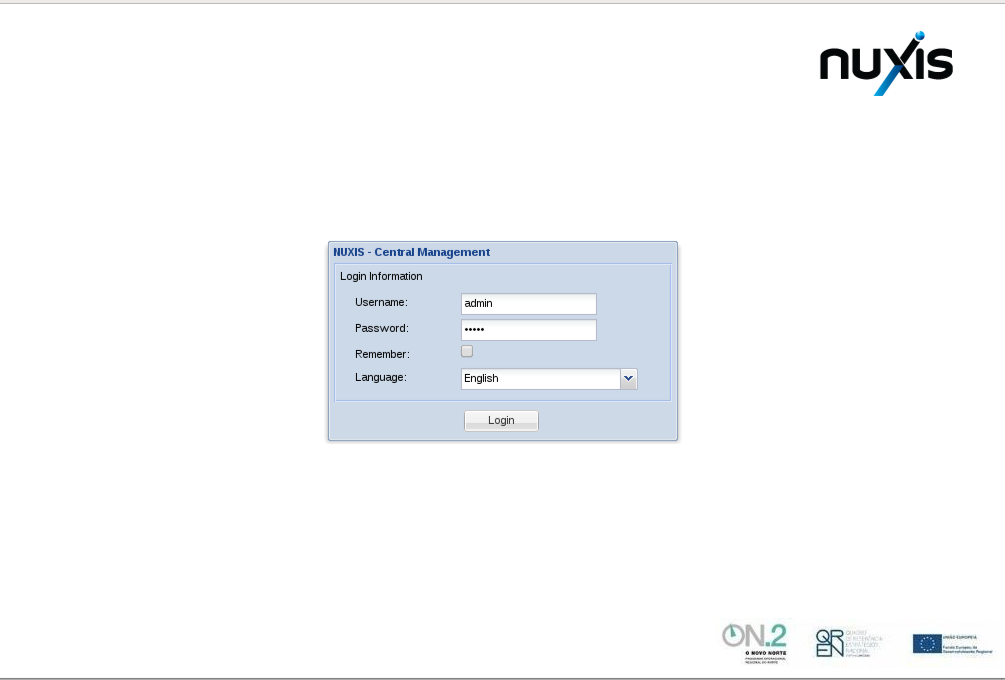
\includegraphics[scale=0.4]{screenshots/install/nuxis/nuxis_enterprise_pos_install_21.png}
    \caption{Configuration after installation - Authentication}
	\label{fig:installation_enterprise_pos_03}
	\end{center}
\end{figure}

Next we access to web inteface with IP address and authentication with user \emph{admin} and default \emph{password} (\emph{admin}).

\begin{figure}[H]
	\begin{center}
    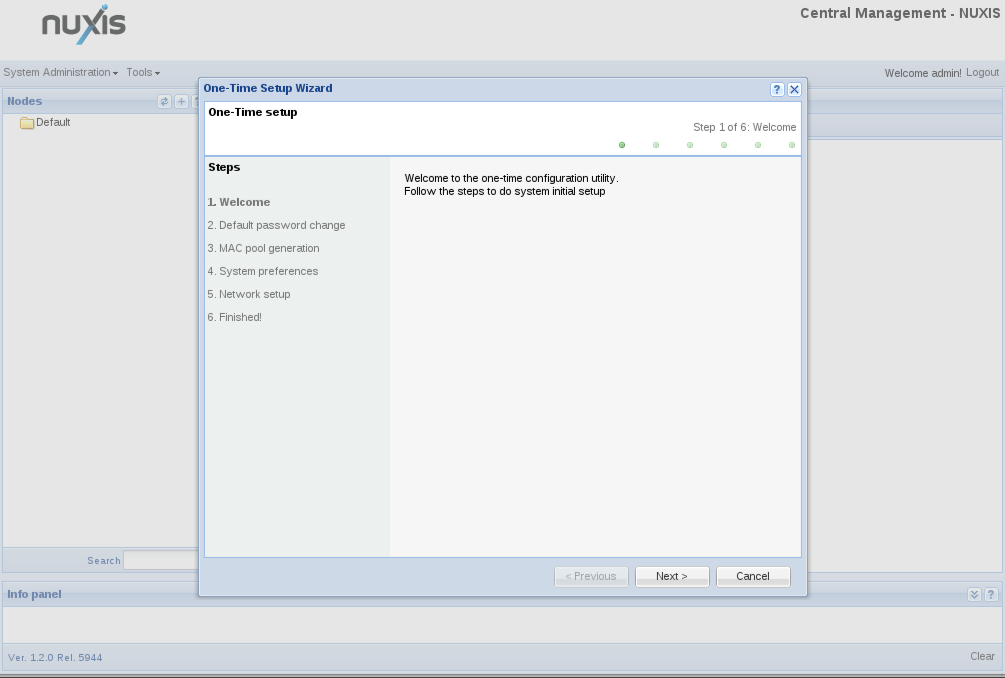
\includegraphics[scale=0.4]{screenshots/install/nuxis/nuxis_enterprise_wiz_install_22.png}
    \caption{Configuration after installation - First time configuration}
	\label{fig:installation_enterprise_wiz_01}
	\end{center}
\end{figure}

On first time configuration, we should change the admin password, generate MAC pool, change conectivity preferences and configure network (see \ref{fig:first_time_wizard}).

\begin{figure}[H]
	\begin{center}
    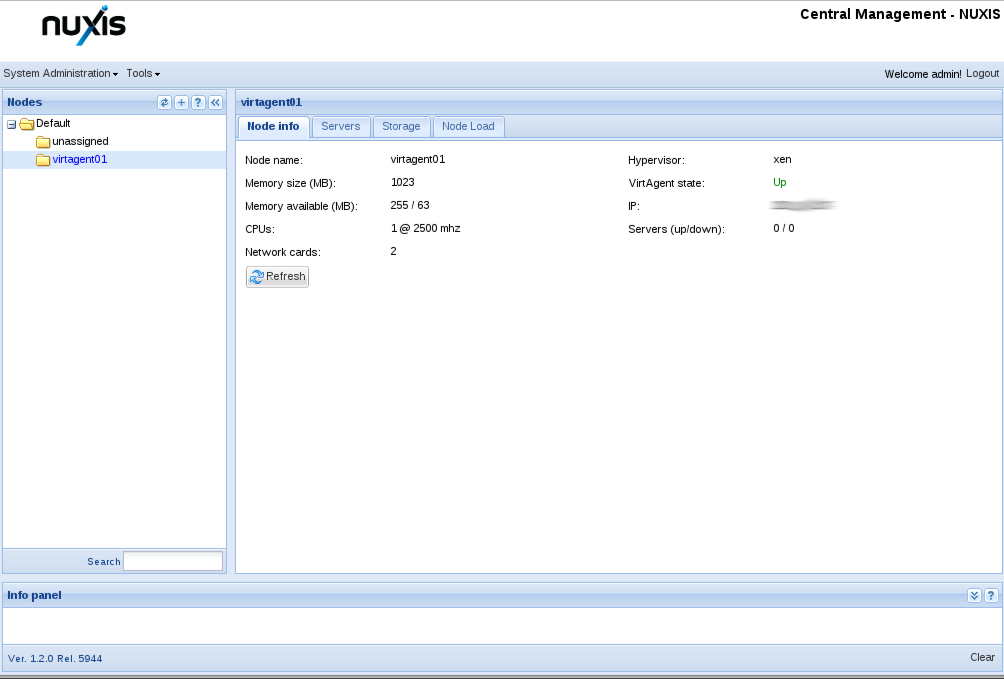
\includegraphics[scale=0.4]{screenshots/install/nuxis/nuxis_enterprise_wiz_install_28.png}
    \caption{Configuration after installation - Virtualization server}
	\label{fig:installation_enterprise_wiz_02}
	\end{center}
\end{figure}

After configure management interface and after install the virtualizations servers, it should be possible to see the servers registered on interface and authorize them (with right click menu) to allow the management.

\pagebreak
